\documentclass[twoside]{book}

% Packages required by doxygen
\usepackage{fixltx2e}
\usepackage{calc}
\usepackage{doxygen}
\usepackage[export]{adjustbox} % also loads graphicx
\usepackage{graphicx}
\usepackage[utf8]{inputenc}
\usepackage{makeidx}
\usepackage{multicol}
\usepackage{multirow}
\PassOptionsToPackage{warn}{textcomp}
\usepackage{textcomp}
\usepackage[nointegrals]{wasysym}
\usepackage[table]{xcolor}

% Font selection
\usepackage[T1]{fontenc}
\usepackage[scaled=.90]{helvet}
\usepackage{courier}
\usepackage{amssymb}
\usepackage{sectsty}
\renewcommand{\familydefault}{\sfdefault}
\allsectionsfont{%
  \fontseries{bc}\selectfont%
  \color{darkgray}%
}
\renewcommand{\DoxyLabelFont}{%
  \fontseries{bc}\selectfont%
  \color{darkgray}%
}
\newcommand{\+}{\discretionary{\mbox{\scriptsize$\hookleftarrow$}}{}{}}

% Page & text layout
\usepackage{geometry}
\geometry{%
  a4paper,%
  top=2.5cm,%
  bottom=2.5cm,%
  left=2.5cm,%
  right=2.5cm%
}
\tolerance=750
\hfuzz=15pt
\hbadness=750
\setlength{\emergencystretch}{15pt}
\setlength{\parindent}{0cm}
\setlength{\parskip}{3ex plus 2ex minus 2ex}
\makeatletter
\renewcommand{\paragraph}{%
  \@startsection{paragraph}{4}{0ex}{-1.0ex}{1.0ex}{%
    \normalfont\normalsize\bfseries\SS@parafont%
  }%
}
\renewcommand{\subparagraph}{%
  \@startsection{subparagraph}{5}{0ex}{-1.0ex}{1.0ex}{%
    \normalfont\normalsize\bfseries\SS@subparafont%
  }%
}
\makeatother

% Headers & footers
\usepackage{fancyhdr}
\pagestyle{fancyplain}
\fancyhead[LE]{\fancyplain{}{\bfseries\thepage}}
\fancyhead[CE]{\fancyplain{}{}}
\fancyhead[RE]{\fancyplain{}{\bfseries\leftmark}}
\fancyhead[LO]{\fancyplain{}{\bfseries\rightmark}}
\fancyhead[CO]{\fancyplain{}{}}
\fancyhead[RO]{\fancyplain{}{\bfseries\thepage}}
\fancyfoot[LE]{\fancyplain{}{}}
\fancyfoot[CE]{\fancyplain{}{}}
\fancyfoot[RE]{\fancyplain{}{\bfseries\scriptsize Generated by Doxygen }}
\fancyfoot[LO]{\fancyplain{}{\bfseries\scriptsize Generated by Doxygen }}
\fancyfoot[CO]{\fancyplain{}{}}
\fancyfoot[RO]{\fancyplain{}{}}
\renewcommand{\footrulewidth}{0.4pt}
\renewcommand{\chaptermark}[1]{%
  \markboth{#1}{}%
}
\renewcommand{\sectionmark}[1]{%
  \markright{\thesection\ #1}%
}

% Indices & bibliography
\usepackage{natbib}
\usepackage[titles]{tocloft}
\setcounter{tocdepth}{3}
\setcounter{secnumdepth}{5}
\makeindex

% Hyperlinks (required, but should be loaded last)
\usepackage{ifpdf}
\ifpdf
  \usepackage[pdftex,pagebackref=true]{hyperref}
\else
  \usepackage[ps2pdf,pagebackref=true]{hyperref}
\fi
\hypersetup{%
  colorlinks=true,%
  linkcolor=blue,%
  citecolor=blue,%
  unicode%
}

% Custom commands
\newcommand{\clearemptydoublepage}{%
  \newpage{\pagestyle{empty}\cleardoublepage}%
}

\usepackage{caption}
\captionsetup{labelsep=space,justification=centering,font={bf},singlelinecheck=off,skip=4pt,position=top}

%===== C O N T E N T S =====

\begin{document}

% Titlepage & ToC
\hypersetup{pageanchor=false,
             bookmarksnumbered=true,
             pdfencoding=unicode
            }
\pagenumbering{alph}
\begin{titlepage}
\vspace*{7cm}
\begin{center}%
{\Large Text\+Editor }\\
\vspace*{1cm}
{\large Generated by Doxygen 1.8.13}\\
\end{center}
\end{titlepage}
\clearemptydoublepage
\pagenumbering{roman}
\tableofcontents
\clearemptydoublepage
\pagenumbering{arabic}
\hypersetup{pageanchor=true}

%--- Begin generated contents ---
\chapter{Hierarchical Index}
\section{Class Hierarchy}
This inheritance list is sorted roughly, but not completely, alphabetically\+:\begin{DoxyCompactList}
\item \contentsline{section}{Editor\+Interface}{\pageref{class_editor_interface}}{}
\item \contentsline{section}{Punctuation\+Mark}{\pageref{class_punctuation_mark}}{}
\item Q\+Main\+Window\begin{DoxyCompactList}
\item \contentsline{section}{Main\+Window}{\pageref{class_main_window}}{}
\end{DoxyCompactList}
\item Q\+Object\begin{DoxyCompactList}
\item \contentsline{section}{Availability}{\pageref{class_availability}}{}
\item \contentsline{section}{Cursor\+Group}{\pageref{class_cursor_group}}{}
\item \contentsline{section}{File\+Status}{\pageref{class_file_status}}{}
\item \contentsline{section}{Plugin\+Manager}{\pageref{class_plugin_manager}}{}
\item \contentsline{section}{Settings\+Manager}{\pageref{class_settings_manager}}{}
\item \contentsline{section}{Theme}{\pageref{class_theme}}{}
\end{DoxyCompactList}
\item Q\+Tab\+Widget\begin{DoxyCompactList}
\item \contentsline{section}{Tab\+Widget}{\pageref{class_tab_widget}}{}
\end{DoxyCompactList}
\item Q\+Undo\+Command\begin{DoxyCompactList}
\item \contentsline{section}{Modify\+Text}{\pageref{class_modify_text}}{}
\end{DoxyCompactList}
\item \contentsline{section}{String\+Manipulator}{\pageref{class_string_manipulator}}{}
\item \contentsline{section}{Text\+High\+Light}{\pageref{class_text_high_light}}{}
\end{DoxyCompactList}

\chapter{Class Index}
\section{Class List}
Here are the classes, structs, unions and interfaces with brief descriptions\+:\begin{DoxyCompactList}
\item\contentsline{section}{\hyperlink{class_availability}{Availability} }{\pageref{class_availability}}{}
\item\contentsline{section}{\hyperlink{class_cursor_group}{Cursor\+Group} }{\pageref{class_cursor_group}}{}
\item\contentsline{section}{\hyperlink{class_editor_interface}{Editor\+Interface} }{\pageref{class_editor_interface}}{}
\item\contentsline{section}{\hyperlink{class_file_status}{File\+Status} }{\pageref{class_file_status}}{}
\item\contentsline{section}{\hyperlink{class_main_window}{Main\+Window} }{\pageref{class_main_window}}{}
\item\contentsline{section}{\hyperlink{class_modify_text}{Modify\+Text} }{\pageref{class_modify_text}}{}
\item\contentsline{section}{\hyperlink{class_plugin_manager}{Plugin\+Manager} }{\pageref{class_plugin_manager}}{}
\item\contentsline{section}{\hyperlink{class_punctuation_mark}{Punctuation\+Mark} }{\pageref{class_punctuation_mark}}{}
\item\contentsline{section}{\hyperlink{class_settings_manager}{Settings\+Manager} }{\pageref{class_settings_manager}}{}
\item\contentsline{section}{\hyperlink{class_string_manipulator}{String\+Manipulator} }{\pageref{class_string_manipulator}}{}
\item\contentsline{section}{\hyperlink{class_tab_widget}{Tab\+Widget} }{\pageref{class_tab_widget}}{}
\item\contentsline{section}{\hyperlink{class_text_high_light}{Text\+High\+Light} }{\pageref{class_text_high_light}}{}
\item\contentsline{section}{\hyperlink{class_theme}{Theme} }{\pageref{class_theme}}{}
\end{DoxyCompactList}

\chapter{Class Documentation}
\hypertarget{class_insert_text}{}\section{Insert\+Text Class Reference}
\label{class_insert_text}\index{Insert\+Text@{Insert\+Text}}
Inheritance diagram for Insert\+Text\+:\begin{figure}[H]
\begin{center}
\leavevmode
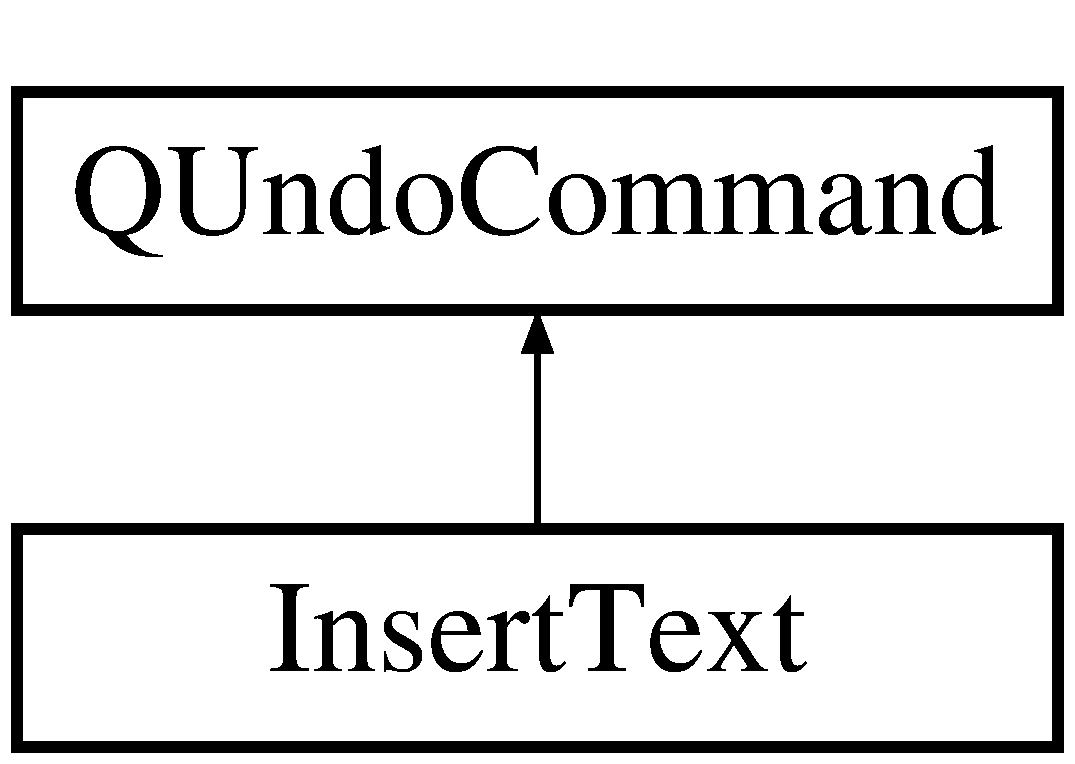
\includegraphics[height=2.000000cm]{class_insert_text}
\end{center}
\end{figure}
\subsection*{Public Member Functions}
\begin{DoxyCompactItemize}
\item 
\mbox{\Hypertarget{class_insert_text_a81753e5c53a97be47b09b2d88ba16cae}\label{class_insert_text_a81753e5c53a97be47b09b2d88ba16cae}} 
{\bfseries Insert\+Text} (Q\+Plain\+Text\+Edit $\ast$editor, const Q\+String \&text, const Q\+String \&delimiter, Q\+Undo\+Command $\ast$parent=nullptr)
\item 
\mbox{\Hypertarget{class_insert_text_a225926a1d60d347575ac77ad47a9f4fe}\label{class_insert_text_a225926a1d60d347575ac77ad47a9f4fe}} 
void {\bfseries undo} () override
\item 
\mbox{\Hypertarget{class_insert_text_adb183bda76ba999719e467097fb17212}\label{class_insert_text_adb183bda76ba999719e467097fb17212}} 
void {\bfseries redo} () override
\end{DoxyCompactItemize}


The documentation for this class was generated from the following files\+:\begin{DoxyCompactItemize}
\item 
/home/laur/\+Desktop/\+Text\+Editor/Insert\+Text.\+h\item 
/home/laur/\+Desktop/\+Text\+Editor/Insert\+Text.\+cpp\end{DoxyCompactItemize}

\hypertarget{class_main_window}{}\section{Main\+Window Class Reference}
\label{class_main_window}\index{Main\+Window@{Main\+Window}}
Inheritance diagram for Main\+Window\+:\begin{figure}[H]
\begin{center}
\leavevmode
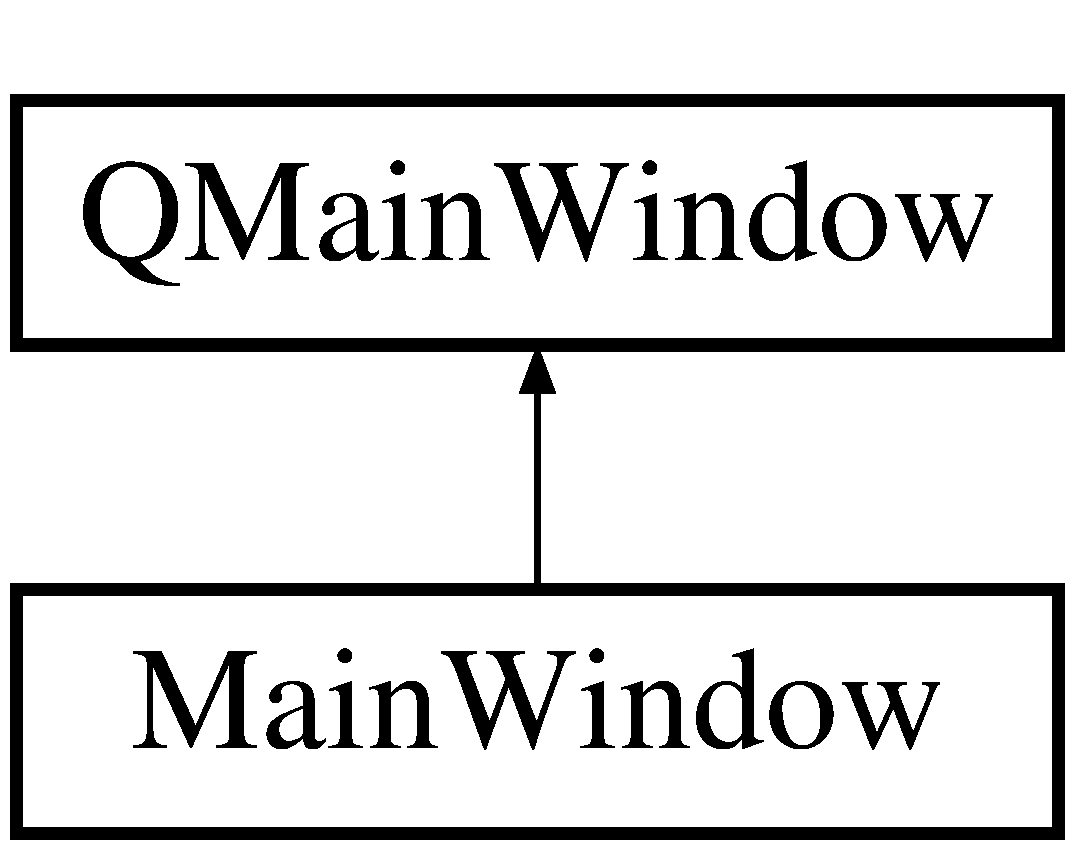
\includegraphics[height=2.000000cm]{class_main_window}
\end{center}
\end{figure}
\subsection*{Public Types}
\begin{DoxyCompactItemize}
\item 
\mbox{\Hypertarget{class_main_window_a084c1dc594e504659ff9e10c7f870bd2}\label{class_main_window_a084c1dc594e504659ff9e10c7f870bd2}} 
enum {\bfseries mode} \{ {\bfseries default\+\_\+mode}, 
{\bfseries dark\+\_\+mode}
 \}
\end{DoxyCompactItemize}
\subsection*{Public Member Functions}
\begin{DoxyCompactItemize}
\item 
\mbox{\Hypertarget{class_main_window_a8b244be8b7b7db1b08de2a2acb9409db}\label{class_main_window_a8b244be8b7b7db1b08de2a2acb9409db}} 
{\bfseries Main\+Window} (Q\+Widget $\ast$parent=0)
\item 
\mbox{\Hypertarget{class_main_window_abf335cb9ff46aa274bc09c331aa5f897}\label{class_main_window_abf335cb9ff46aa274bc09c331aa5f897}} 
void {\bfseries set\+High\+Light} (const \hyperlink{class_text_high_light}{Text\+High\+Light} \&highlight, const int required\+Format=colored\+\_\+format)
\item 
\mbox{\Hypertarget{class_main_window_a35ffd96169163c809eb8c11f2dedda28}\label{class_main_window_a35ffd96169163c809eb8c11f2dedda28}} 
void {\bfseries modify\+Text} (int($\ast$function)(std\+::string \&text))
\item 
\mbox{\Hypertarget{class_main_window_a28f0773e43cc100fa5dc6019b09780bb}\label{class_main_window_a28f0773e43cc100fa5dc6019b09780bb}} 
void {\bfseries change\+Dates\+In\+Text} (const String\+Manipulator\+::date\+Format format)
\item 
\mbox{\Hypertarget{class_main_window_a059e8c7deed9f985c6396182779590f2}\label{class_main_window_a059e8c7deed9f985c6396182779590f2}} 
void {\bfseries set\+Appearance} (mode selected\+\_\+mode)
\item 
\mbox{\Hypertarget{class_main_window_a6cdeb56a312f6b1935436e6203912c09}\label{class_main_window_a6cdeb56a312f6b1935436e6203912c09}} 
Q\+Plain\+Text\+Edit $\ast$ {\bfseries get\+Current\+Text\+Edit} ()
\item 
\mbox{\Hypertarget{class_main_window_a61d74ea396ffe9c23581f19a3e8368af}\label{class_main_window_a61d74ea396ffe9c23581f19a3e8368af}} 
Q\+Plain\+Text\+Edit $\ast$ {\bfseries get\+Text\+Edit\+By\+Name} (const Q\+String \&name)
\end{DoxyCompactItemize}


The documentation for this class was generated from the following files\+:\begin{DoxyCompactItemize}
\item 
/home/laur/\+Desktop/\+Text\+Editor/mainwindow.\+h\item 
/home/laur/\+Desktop/\+Text\+Editor/mainwindow.\+cpp\end{DoxyCompactItemize}

\hypertarget{class_modify_text}{}\section{Modify\+Text Class Reference}
\label{class_modify_text}\index{Modify\+Text@{Modify\+Text}}
Inheritance diagram for Modify\+Text\+:\begin{figure}[H]
\begin{center}
\leavevmode
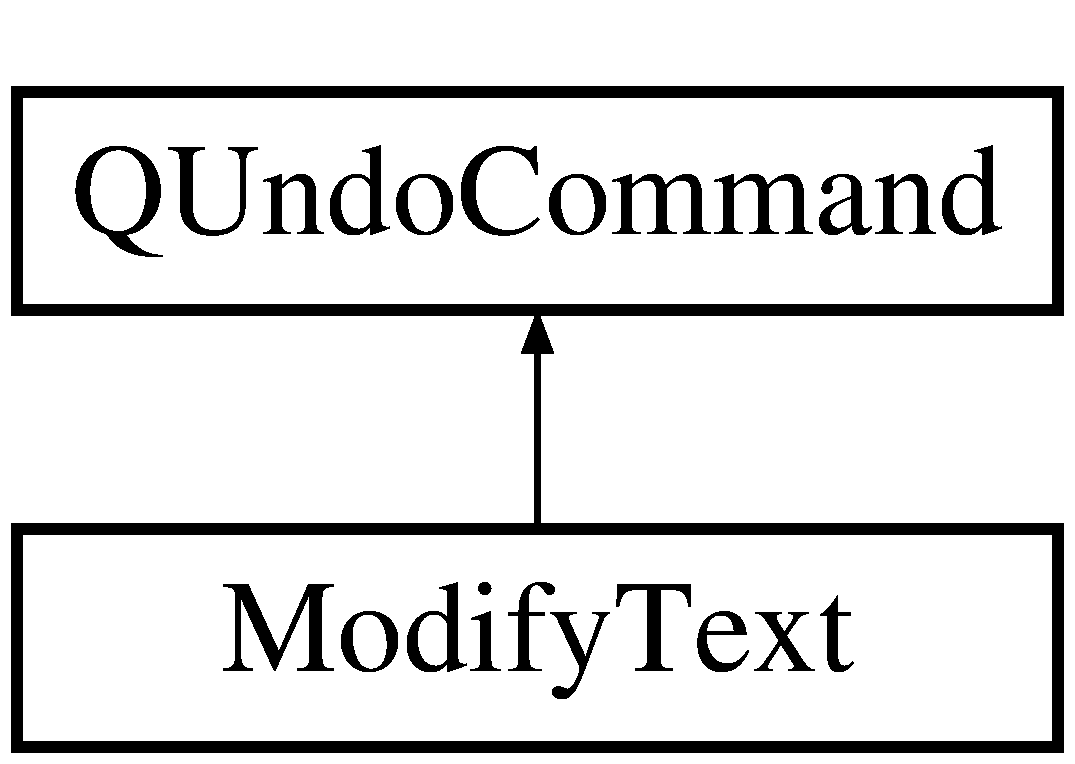
\includegraphics[height=2.000000cm]{class_modify_text}
\end{center}
\end{figure}
\subsection*{Public Member Functions}
\begin{DoxyCompactItemize}
\item 
\mbox{\Hypertarget{class_modify_text_a1b4735d4eeb33f9ef88cf3f33b5e8723}\label{class_modify_text_a1b4735d4eeb33f9ef88cf3f33b5e8723}} 
{\bfseries Modify\+Text} (Q\+Plain\+Text\+Edit $\ast$editor, const Q\+String \&old\+Text, const Q\+String \&new\+Text, Q\+Undo\+Command $\ast$parent=nullptr)
\item 
\mbox{\Hypertarget{class_modify_text_ac6f267ca4f2d3e6dd862975268291dab}\label{class_modify_text_ac6f267ca4f2d3e6dd862975268291dab}} 
void {\bfseries undo} () override
\item 
\mbox{\Hypertarget{class_modify_text_acf0fe8ee7ad397b66c012afe2aa1999d}\label{class_modify_text_acf0fe8ee7ad397b66c012afe2aa1999d}} 
void {\bfseries redo} () override
\end{DoxyCompactItemize}


The documentation for this class was generated from the following files\+:\begin{DoxyCompactItemize}
\item 
/home/laur/\+Desktop/\+Text\+Editor/Modify\+Text.\+h\item 
/home/laur/\+Desktop/\+Text\+Editor/Modify\+Text.\+cpp\end{DoxyCompactItemize}

\hypertarget{class_punctuation_mark}{}\section{Punctuation\+Mark Class Reference}
\label{class_punctuation_mark}\index{Punctuation\+Mark@{Punctuation\+Mark}}
\subsection*{Static Public Member Functions}
\begin{DoxyCompactItemize}
\item 
\mbox{\Hypertarget{class_punctuation_mark_ab46bc081295e69d79097344be31fa4bc}\label{class_punctuation_mark_ab46bc081295e69d79097344be31fa4bc}} 
static bool {\bfseries is\+Mark} (const char character)
\item 
\mbox{\Hypertarget{class_punctuation_mark_ac1f9081cafe0c3290a32da66bddff6b9}\label{class_punctuation_mark_ac1f9081cafe0c3290a32da66bddff6b9}} 
static std\+::vector$<$ int $>$ {\bfseries search\+For} (const char character, const std\+::string \&text)
\item 
\mbox{\Hypertarget{class_punctuation_mark_aef43138e26ce10d11728047f46c78fde}\label{class_punctuation_mark_aef43138e26ce10d11728047f46c78fde}} 
static std\+::vector$<$ int $>$ {\bfseries find\+All\+Marks} (const std\+::string \&text)
\end{DoxyCompactItemize}
\subsection*{Static Public Attributes}
\begin{DoxyCompactItemize}
\item 
\mbox{\Hypertarget{class_punctuation_mark_a4c6e2bf50dfbfdb36e6c3051b740c468}\label{class_punctuation_mark_a4c6e2bf50dfbfdb36e6c3051b740c468}} 
static std\+::vector$<$ char $>$ const {\bfseries marks} \{\textquotesingle{}.\textquotesingle{},\textquotesingle{},\textquotesingle{},\textquotesingle{}!\textquotesingle{},\textquotesingle{}?\textquotesingle{},\textquotesingle{}(\textquotesingle{},\textquotesingle{})\textquotesingle{},\textquotesingle{}\mbox{[}\textquotesingle{},\textquotesingle{}\mbox{]}\textquotesingle{},\textquotesingle{}\{\textquotesingle{},\textquotesingle{}\}\textquotesingle{},\textquotesingle{}\+:\textquotesingle{}\}
\end{DoxyCompactItemize}


The documentation for this class was generated from the following files\+:\begin{DoxyCompactItemize}
\item 
/home/laur/\+Desktop/\+Text\+Editor/Punctuation\+Mark.\+h\item 
/home/laur/\+Desktop/\+Text\+Editor/Punctuation\+Mark.\+cpp\end{DoxyCompactItemize}

\hypertarget{class_string_manipulator}{}\section{String\+Manipulator Class Reference}
\label{class_string_manipulator}\index{String\+Manipulator@{String\+Manipulator}}
\subsection*{Public Types}
\begin{DoxyCompactItemize}
\item 
\mbox{\Hypertarget{class_string_manipulator_a334eebb23cccec56948656326507617e}\label{class_string_manipulator_a334eebb23cccec56948656326507617e}} 
enum {\bfseries date\+Format} \{ \newline
{\bfseries slash\+\_\+big\+\_\+endian}, 
{\bfseries slash\+\_\+little\+\_\+endian}, 
{\bfseries dot\+\_\+big\+\_\+endian}, 
{\bfseries dot\+\_\+little\+\_\+endian}, 
\newline
{\bfseries line\+\_\+big\+\_\+endian}, 
{\bfseries line\+\_\+little\+\_\+endian}
 \}
\end{DoxyCompactItemize}
\subsection*{Static Public Member Functions}
\begin{DoxyCompactItemize}
\item 
static std\+::vector$<$ \hyperlink{class_text_high_light}{Text\+High\+Light} $>$ \hyperlink{class_string_manipulator_adab4023d6e1e822008e3832c56e47d56}{find} (const Q\+String \&pattern, const Q\+String \&text, const bool is\+Regex=false, const Q\+String flag=\char`\"{}A\+LL\char`\"{})
\item 
static \hyperlink{class_text_high_light}{Text\+High\+Light} \hyperlink{class_string_manipulator_a20fdffe83624dbaf91d2f26e79417bed}{replace} (const Q\+String \&replacement, const \hyperlink{class_text_high_light}{Text\+High\+Light} \&highlight, Q\+String \&text)
\item 
static int \hyperlink{class_string_manipulator_a7a77d58ba2445a871cc716a8870f7244}{replace\+All} (const Q\+String \&to\+Replace, const Q\+String \&replacement, Q\+String \&text)
\item 
static int \hyperlink{class_string_manipulator_a254924bbc9bead53372a393aee9f8711}{trim} (Q\+String \&text)
\item 
static int \hyperlink{class_string_manipulator_ac669121dd3e5fda9b8723593fc7ca04d}{padding} (Q\+String \&text)
\item 
static int \hyperlink{class_string_manipulator_ad5ff80ae462045bc6d8f2be32c0da4bb}{capitalize\+All} (Q\+String \&text)
\item 
static int \hyperlink{class_string_manipulator_a0dddee858bb0c58c63fd122645114bcb}{capitalize\+First\+Letter} (Q\+String \&text)
\item 
static int \hyperlink{class_string_manipulator_a236181c606edff1c577a9a88ddb8d7d9}{capitalize\+Offset} (Q\+String \&text, const \hyperlink{class_text_high_light}{Text\+High\+Light} highlight)
\item 
static int \hyperlink{class_string_manipulator_a102944c73c7fc265e426bc7749907e8c}{lowercase\+All} (Q\+String \&text)
\item 
static int \hyperlink{class_string_manipulator_a09536b194993d10f361459873c727c3b}{lowercase\+First\+Letter} (Q\+String \&text)
\item 
static int \hyperlink{class_string_manipulator_ad8075d783befd76e2f456ff1ada8b0f6}{lowercase\+Offset} (Q\+String \&text, const \hyperlink{class_text_high_light}{Text\+High\+Light} \&highlight)
\item 
static int \hyperlink{class_string_manipulator_ae91d0a9b920ae7621a9d49bc2286235a}{transform\+To\+A\+S\+C\+II} (Q\+String \&text)
\item 
static int \hyperlink{class_string_manipulator_ac35afff547abbd79b54b514e2d752a71}{change\+Date\+Format} (Q\+String \&text, date\+Format format)
\item 
static int \hyperlink{class_string_manipulator_a9a6742faa577c63df0725af492b785f7}{find\+Non\+A\+S\+C\+II} (const Q\+String \&text)
\item 
static bool \hyperlink{class_string_manipulator_af0ba293accd9ddf0b7db3973edaa093f}{is\+A\+Date} (const Q\+String \&text)
\item 
static bool \hyperlink{class_string_manipulator_abfc77e41e2b96d37e07fa87cb71bd6da}{is\+A\+Capital\+Letter} (const Q\+Char \&character)
\item 
static bool \hyperlink{class_string_manipulator_a7c6339b8e0f43102fd4b8505fca0530d}{is\+A\+Lowercase\+Letter} (const Q\+Char \&character)
\item 
static bool \hyperlink{class_string_manipulator_a7deb1f37fd0efd4eddfb4cef8ed6eca6}{is\+Letter} (const Q\+Char \&character)
\item 
static bool \hyperlink{class_string_manipulator_af3dc83218b174085453f06453b93d17b}{is\+Number} (const Q\+Char \&character)
\item 
static bool \hyperlink{class_string_manipulator_a51dc44388aac908904aa0408e73ab615}{is\+Regex\+Operator} (const Q\+Char \&character)
\item 
static void \hyperlink{class_string_manipulator_a1bb8e6892955d05c68d523b985bad0bc}{treating\+Exceptions\+For\+Text} (const Q\+String \&text)
\item 
static void \hyperlink{class_string_manipulator_a3892dd94b5a1f6c61736fb523bd6a3ab}{treating\+Exceptions\+For\+Highlight} (const Q\+String \&text, const \hyperlink{class_text_high_light}{Text\+High\+Light} \&highlight)
\item 
static Q\+List$<$ Q\+Char $>$ \hyperlink{class_string_manipulator_a5ac671799b00b71f236dcfb68077cdce}{regex\+Special\+Characters} ()
\item 
static int \hyperlink{class_string_manipulator_af2041957b6df343d55d1cd99719e0d16}{repeal\+Operators} (Q\+String \&text)
\end{DoxyCompactItemize}


\subsection{Member Function Documentation}
\mbox{\Hypertarget{class_string_manipulator_ad5ff80ae462045bc6d8f2be32c0da4bb}\label{class_string_manipulator_ad5ff80ae462045bc6d8f2be32c0da4bb}} 
\index{String\+Manipulator@{String\+Manipulator}!capitalize\+All@{capitalize\+All}}
\index{capitalize\+All@{capitalize\+All}!String\+Manipulator@{String\+Manipulator}}
\subsubsection{\texorpdfstring{capitalize\+All()}{capitalizeAll()}}
{\footnotesize\ttfamily int String\+Manipulator\+::capitalize\+All (\begin{DoxyParamCaption}\item[{Q\+String \&}]{text }\end{DoxyParamCaption})\hspace{0.3cm}{\ttfamily [static]}}

Transforma toate literele mici din text in majuscule


\begin{DoxyParams}[1]{Parameters}
\mbox{\tt in}  & {\em } & \\
\hline
\end{DoxyParams}
\mbox{\Hypertarget{class_string_manipulator_a0dddee858bb0c58c63fd122645114bcb}\label{class_string_manipulator_a0dddee858bb0c58c63fd122645114bcb}} 
\index{String\+Manipulator@{String\+Manipulator}!capitalize\+First\+Letter@{capitalize\+First\+Letter}}
\index{capitalize\+First\+Letter@{capitalize\+First\+Letter}!String\+Manipulator@{String\+Manipulator}}
\subsubsection{\texorpdfstring{capitalize\+First\+Letter()}{capitalizeFirstLetter()}}
{\footnotesize\ttfamily int String\+Manipulator\+::capitalize\+First\+Letter (\begin{DoxyParamCaption}\item[{Q\+String \&}]{text }\end{DoxyParamCaption})\hspace{0.3cm}{\ttfamily [static]}}

Transforma la i nmajuscula fiecare litera mica la inceputul unei propozitii


\begin{DoxyParams}[1]{Parameters}
\mbox{\tt in}  & {\em } & \\
\hline
\end{DoxyParams}
\mbox{\Hypertarget{class_string_manipulator_a236181c606edff1c577a9a88ddb8d7d9}\label{class_string_manipulator_a236181c606edff1c577a9a88ddb8d7d9}} 
\index{String\+Manipulator@{String\+Manipulator}!capitalize\+Offset@{capitalize\+Offset}}
\index{capitalize\+Offset@{capitalize\+Offset}!String\+Manipulator@{String\+Manipulator}}
\subsubsection{\texorpdfstring{capitalize\+Offset()}{capitalizeOffset()}}
{\footnotesize\ttfamily int String\+Manipulator\+::capitalize\+Offset (\begin{DoxyParamCaption}\item[{Q\+String \&}]{text,  }\item[{const \hyperlink{class_text_high_light}{Text\+High\+Light}}]{highlight }\end{DoxyParamCaption})\hspace{0.3cm}{\ttfamily [static]}}

Transforma in majuscule literele mici din secventa specificata de highlight


\begin{DoxyParams}[1]{Parameters}
\mbox{\tt in}  & {\em } & \\
\hline
\end{DoxyParams}
\mbox{\Hypertarget{class_string_manipulator_ac35afff547abbd79b54b514e2d752a71}\label{class_string_manipulator_ac35afff547abbd79b54b514e2d752a71}} 
\index{String\+Manipulator@{String\+Manipulator}!change\+Date\+Format@{change\+Date\+Format}}
\index{change\+Date\+Format@{change\+Date\+Format}!String\+Manipulator@{String\+Manipulator}}
\subsubsection{\texorpdfstring{change\+Date\+Format()}{changeDateFormat()}}
{\footnotesize\ttfamily int String\+Manipulator\+::change\+Date\+Format (\begin{DoxyParamCaption}\item[{Q\+String \&}]{text,  }\item[{date\+Format}]{format }\end{DoxyParamCaption})\hspace{0.3cm}{\ttfamily [static]}}

Transforma formatul de data din textul dat in formatul dorit


\begin{DoxyParams}[1]{Parameters}
\mbox{\tt in}  & {\em } & \\
\hline
\end{DoxyParams}
\mbox{\Hypertarget{class_string_manipulator_adab4023d6e1e822008e3832c56e47d56}\label{class_string_manipulator_adab4023d6e1e822008e3832c56e47d56}} 
\index{String\+Manipulator@{String\+Manipulator}!find@{find}}
\index{find@{find}!String\+Manipulator@{String\+Manipulator}}
\subsubsection{\texorpdfstring{find()}{find()}}
{\footnotesize\ttfamily std\+::vector$<$ \hyperlink{class_text_high_light}{Text\+High\+Light} $>$ String\+Manipulator\+::find (\begin{DoxyParamCaption}\item[{const Q\+String \&}]{pattern,  }\item[{const Q\+String \&}]{text,  }\item[{const bool}]{is\+Regex = {\ttfamily false},  }\item[{const Q\+String}]{flag = {\ttfamily \char`\"{}ALL\char`\"{}} }\end{DoxyParamCaption})\hspace{0.3cm}{\ttfamily [static]}}

Cauta in textul dat secvente de text corespunzatoare sablonului pattern 
\begin{DoxyParams}[1]{Parameters}
\mbox{\tt in}  & {\em pattern} & -\/ sablonul cautarii -\/ poate fi o secventa simpla de text sau o expresie regulata \\
\hline
\mbox{\tt in}  & {\em text} & -\/ textul in care se cauta sablonul \\
\hline
\mbox{\tt in}  & {\em is\+Regex} & -\/flag ce indica daca sablonul este o expresie regulata sau nu\\
\hline
\end{DoxyParams}
\begin{DoxyReturn}{Returns}
un vector cu pozitiile si lungimile rezultatelor cautarii 
\end{DoxyReturn}
\mbox{\Hypertarget{class_string_manipulator_a9a6742faa577c63df0725af492b785f7}\label{class_string_manipulator_a9a6742faa577c63df0725af492b785f7}} 
\index{String\+Manipulator@{String\+Manipulator}!find\+Non\+A\+S\+C\+II@{find\+Non\+A\+S\+C\+II}}
\index{find\+Non\+A\+S\+C\+II@{find\+Non\+A\+S\+C\+II}!String\+Manipulator@{String\+Manipulator}}
\subsubsection{\texorpdfstring{find\+Non\+A\+S\+C\+I\+I()}{findNonASCII()}}
{\footnotesize\ttfamily int String\+Manipulator\+::find\+Non\+A\+S\+C\+II (\begin{DoxyParamCaption}\item[{const Q\+String \&}]{text }\end{DoxyParamCaption})\hspace{0.3cm}{\ttfamily [static]}}

gaseste prima pozitie a unui caracter non-\/\+A\+S\+C\+II


\begin{DoxyParams}[1]{Parameters}
\mbox{\tt in}  & {\em text} & -\/ textul ce trebuie verificat\\
\hline
\end{DoxyParams}
\begin{DoxyReturn}{Returns}
prima pozitie a unui caracter non-\/\+A\+S\+C\+II 
\end{DoxyReturn}
\mbox{\Hypertarget{class_string_manipulator_abfc77e41e2b96d37e07fa87cb71bd6da}\label{class_string_manipulator_abfc77e41e2b96d37e07fa87cb71bd6da}} 
\index{String\+Manipulator@{String\+Manipulator}!is\+A\+Capital\+Letter@{is\+A\+Capital\+Letter}}
\index{is\+A\+Capital\+Letter@{is\+A\+Capital\+Letter}!String\+Manipulator@{String\+Manipulator}}
\subsubsection{\texorpdfstring{is\+A\+Capital\+Letter()}{isACapitalLetter()}}
{\footnotesize\ttfamily bool String\+Manipulator\+::is\+A\+Capital\+Letter (\begin{DoxyParamCaption}\item[{const Q\+Char \&}]{character }\end{DoxyParamCaption})\hspace{0.3cm}{\ttfamily [static]}}

specifica daca caracterul dat este majuscula sau nu


\begin{DoxyParams}[1]{Parameters}
\mbox{\tt in}  & {\em character} & -\/ caracterul de verificat\\
\hline
\end{DoxyParams}
\begin{DoxyReturn}{Returns}
true daca e majuscula, false in caz contrar 
\end{DoxyReturn}
\mbox{\Hypertarget{class_string_manipulator_af0ba293accd9ddf0b7db3973edaa093f}\label{class_string_manipulator_af0ba293accd9ddf0b7db3973edaa093f}} 
\index{String\+Manipulator@{String\+Manipulator}!is\+A\+Date@{is\+A\+Date}}
\index{is\+A\+Date@{is\+A\+Date}!String\+Manipulator@{String\+Manipulator}}
\subsubsection{\texorpdfstring{is\+A\+Date()}{isADate()}}
{\footnotesize\ttfamily bool String\+Manipulator\+::is\+A\+Date (\begin{DoxyParamCaption}\item[{const Q\+String \&}]{text }\end{DoxyParamCaption})\hspace{0.3cm}{\ttfamily [static]}}

specifica daca textul dat este un format de data cunoscut


\begin{DoxyParams}[1]{Parameters}
\mbox{\tt in}  & {\em text} & -\/ textul ce trebuie verificat\\
\hline
\end{DoxyParams}
\begin{DoxyReturn}{Returns}
true daca este un format si false daca nu respecta nici un format 
\end{DoxyReturn}
\mbox{\Hypertarget{class_string_manipulator_a7c6339b8e0f43102fd4b8505fca0530d}\label{class_string_manipulator_a7c6339b8e0f43102fd4b8505fca0530d}} 
\index{String\+Manipulator@{String\+Manipulator}!is\+A\+Lowercase\+Letter@{is\+A\+Lowercase\+Letter}}
\index{is\+A\+Lowercase\+Letter@{is\+A\+Lowercase\+Letter}!String\+Manipulator@{String\+Manipulator}}
\subsubsection{\texorpdfstring{is\+A\+Lowercase\+Letter()}{isALowercaseLetter()}}
{\footnotesize\ttfamily bool String\+Manipulator\+::is\+A\+Lowercase\+Letter (\begin{DoxyParamCaption}\item[{const Q\+Char \&}]{character }\end{DoxyParamCaption})\hspace{0.3cm}{\ttfamily [static]}}

specifica daca caracterul dat este litera mica sau nu


\begin{DoxyParams}[1]{Parameters}
\mbox{\tt in}  & {\em the} & character\\
\hline
\end{DoxyParams}
\begin{DoxyReturn}{Returns}
true daca caracterul este litera mica, false in caz contrar 
\end{DoxyReturn}
\mbox{\Hypertarget{class_string_manipulator_a7deb1f37fd0efd4eddfb4cef8ed6eca6}\label{class_string_manipulator_a7deb1f37fd0efd4eddfb4cef8ed6eca6}} 
\index{String\+Manipulator@{String\+Manipulator}!is\+Letter@{is\+Letter}}
\index{is\+Letter@{is\+Letter}!String\+Manipulator@{String\+Manipulator}}
\subsubsection{\texorpdfstring{is\+Letter()}{isLetter()}}
{\footnotesize\ttfamily bool String\+Manipulator\+::is\+Letter (\begin{DoxyParamCaption}\item[{const Q\+Char \&}]{character }\end{DoxyParamCaption})\hspace{0.3cm}{\ttfamily [static]}}

specifica daca caracterul dat este o litera sau nu


\begin{DoxyParams}[1]{Parameters}
\mbox{\tt in}  & {\em character} & -\/ caracterul ce trebuie verificat\\
\hline
\end{DoxyParams}
\begin{DoxyReturn}{Returns}
true daca caracterul este litera, false in caz contrar 
\end{DoxyReturn}
\mbox{\Hypertarget{class_string_manipulator_af3dc83218b174085453f06453b93d17b}\label{class_string_manipulator_af3dc83218b174085453f06453b93d17b}} 
\index{String\+Manipulator@{String\+Manipulator}!is\+Number@{is\+Number}}
\index{is\+Number@{is\+Number}!String\+Manipulator@{String\+Manipulator}}
\subsubsection{\texorpdfstring{is\+Number()}{isNumber()}}
{\footnotesize\ttfamily bool String\+Manipulator\+::is\+Number (\begin{DoxyParamCaption}\item[{const Q\+Char \&}]{character }\end{DoxyParamCaption})\hspace{0.3cm}{\ttfamily [static]}}

specifica daca caracterul dat este o cifra sau nu


\begin{DoxyParams}[1]{Parameters}
\mbox{\tt in}  & {\em character} & -\/ caracterul ce trebuie verificat\\
\hline
\end{DoxyParams}
\begin{DoxyReturn}{Returns}
true daca este cifra, false in caz contrar 
\end{DoxyReturn}
\mbox{\Hypertarget{class_string_manipulator_a51dc44388aac908904aa0408e73ab615}\label{class_string_manipulator_a51dc44388aac908904aa0408e73ab615}} 
\index{String\+Manipulator@{String\+Manipulator}!is\+Regex\+Operator@{is\+Regex\+Operator}}
\index{is\+Regex\+Operator@{is\+Regex\+Operator}!String\+Manipulator@{String\+Manipulator}}
\subsubsection{\texorpdfstring{is\+Regex\+Operator()}{isRegexOperator()}}
{\footnotesize\ttfamily bool String\+Manipulator\+::is\+Regex\+Operator (\begin{DoxyParamCaption}\item[{const Q\+Char \&}]{character }\end{DoxyParamCaption})\hspace{0.3cm}{\ttfamily [static]}}

verifica daca caracterul primut ca intrare este un construct regex


\begin{DoxyParams}[1]{Parameters}
\mbox{\tt in}  & {\em character} & -\/ caracterul care trebuie verificat\\
\hline
\end{DoxyParams}
\begin{DoxyReturn}{Returns}
-\/ true daca caracterul este un construct regex si false in caz contrar 
\end{DoxyReturn}
\mbox{\Hypertarget{class_string_manipulator_a102944c73c7fc265e426bc7749907e8c}\label{class_string_manipulator_a102944c73c7fc265e426bc7749907e8c}} 
\index{String\+Manipulator@{String\+Manipulator}!lowercase\+All@{lowercase\+All}}
\index{lowercase\+All@{lowercase\+All}!String\+Manipulator@{String\+Manipulator}}
\subsubsection{\texorpdfstring{lowercase\+All()}{lowercaseAll()}}
{\footnotesize\ttfamily int String\+Manipulator\+::lowercase\+All (\begin{DoxyParamCaption}\item[{Q\+String \&}]{text }\end{DoxyParamCaption})\hspace{0.3cm}{\ttfamily [static]}}

Transforma in litere mici toate majusculele din text


\begin{DoxyParams}[1]{Parameters}
\mbox{\tt in}  & {\em } & \\
\hline
\end{DoxyParams}
\mbox{\Hypertarget{class_string_manipulator_a09536b194993d10f361459873c727c3b}\label{class_string_manipulator_a09536b194993d10f361459873c727c3b}} 
\index{String\+Manipulator@{String\+Manipulator}!lowercase\+First\+Letter@{lowercase\+First\+Letter}}
\index{lowercase\+First\+Letter@{lowercase\+First\+Letter}!String\+Manipulator@{String\+Manipulator}}
\subsubsection{\texorpdfstring{lowercase\+First\+Letter()}{lowercaseFirstLetter()}}
{\footnotesize\ttfamily int String\+Manipulator\+::lowercase\+First\+Letter (\begin{DoxyParamCaption}\item[{Q\+String \&}]{text }\end{DoxyParamCaption})\hspace{0.3cm}{\ttfamily [static]}}

Functia opusa functiei capitalize\+First\+Letter /// 
\begin{DoxyParams}[1]{Parameters}
\mbox{\tt in}  & {\em } & \\
\hline
\end{DoxyParams}
\mbox{\Hypertarget{class_string_manipulator_ad8075d783befd76e2f456ff1ada8b0f6}\label{class_string_manipulator_ad8075d783befd76e2f456ff1ada8b0f6}} 
\index{String\+Manipulator@{String\+Manipulator}!lowercase\+Offset@{lowercase\+Offset}}
\index{lowercase\+Offset@{lowercase\+Offset}!String\+Manipulator@{String\+Manipulator}}
\subsubsection{\texorpdfstring{lowercase\+Offset()}{lowercaseOffset()}}
{\footnotesize\ttfamily int String\+Manipulator\+::lowercase\+Offset (\begin{DoxyParamCaption}\item[{Q\+String \&}]{text,  }\item[{const \hyperlink{class_text_high_light}{Text\+High\+Light} \&}]{highlight }\end{DoxyParamCaption})\hspace{0.3cm}{\ttfamily [static]}}

Transforma in litere mici toate majusculele din text specificate de highlight


\begin{DoxyParams}[1]{Parameters}
\mbox{\tt in}  & {\em } & \\
\hline
\end{DoxyParams}
\mbox{\Hypertarget{class_string_manipulator_ac669121dd3e5fda9b8723593fc7ca04d}\label{class_string_manipulator_ac669121dd3e5fda9b8723593fc7ca04d}} 
\index{String\+Manipulator@{String\+Manipulator}!padding@{padding}}
\index{padding@{padding}!String\+Manipulator@{String\+Manipulator}}
\subsubsection{\texorpdfstring{padding()}{padding()}}
{\footnotesize\ttfamily int String\+Manipulator\+::padding (\begin{DoxyParamCaption}\item[{Q\+String \&}]{text }\end{DoxyParamCaption})\hspace{0.3cm}{\ttfamily [static]}}

Completeaza cu spatii in zonele unde ar trebui sa existe. Zone tinta\+: Intre propozitii, dupa semnul de punctuatie sau dupa fiecare virgula


\begin{DoxyParams}[1]{Parameters}
\mbox{\tt in}  & {\em } & \\
\hline
\end{DoxyParams}
\mbox{\Hypertarget{class_string_manipulator_a5ac671799b00b71f236dcfb68077cdce}\label{class_string_manipulator_a5ac671799b00b71f236dcfb68077cdce}} 
\index{String\+Manipulator@{String\+Manipulator}!regex\+Special\+Characters@{regex\+Special\+Characters}}
\index{regex\+Special\+Characters@{regex\+Special\+Characters}!String\+Manipulator@{String\+Manipulator}}
\subsubsection{\texorpdfstring{regex\+Special\+Characters()}{regexSpecialCharacters()}}
{\footnotesize\ttfamily Q\+List$<$ Q\+Char $>$ String\+Manipulator\+::regex\+Special\+Characters (\begin{DoxyParamCaption}{ }\end{DoxyParamCaption})\hspace{0.3cm}{\ttfamily [static]}}

\begin{DoxyReturn}{Returns}
o lista cu caractere ce reprezinta operatori regex 
\end{DoxyReturn}
\mbox{\Hypertarget{class_string_manipulator_af2041957b6df343d55d1cd99719e0d16}\label{class_string_manipulator_af2041957b6df343d55d1cd99719e0d16}} 
\index{String\+Manipulator@{String\+Manipulator}!repeal\+Operators@{repeal\+Operators}}
\index{repeal\+Operators@{repeal\+Operators}!String\+Manipulator@{String\+Manipulator}}
\subsubsection{\texorpdfstring{repeal\+Operators()}{repealOperators()}}
{\footnotesize\ttfamily int String\+Manipulator\+::repeal\+Operators (\begin{DoxyParamCaption}\item[{Q\+String \&}]{text }\end{DoxyParamCaption})\hspace{0.3cm}{\ttfamily [static]}}

in cazul in care expresia ce trebuie gasita contine operatori de tip regex, se introduce caracterul \char`\"{}\textbackslash{}\char`\"{} pentru a le anula efectul


\begin{DoxyParams}[1]{Parameters}
\mbox{\tt in}  & {\em } & \\
\hline
\end{DoxyParams}
\mbox{\Hypertarget{class_string_manipulator_a20fdffe83624dbaf91d2f26e79417bed}\label{class_string_manipulator_a20fdffe83624dbaf91d2f26e79417bed}} 
\index{String\+Manipulator@{String\+Manipulator}!replace@{replace}}
\index{replace@{replace}!String\+Manipulator@{String\+Manipulator}}
\subsubsection{\texorpdfstring{replace()}{replace()}}
{\footnotesize\ttfamily \hyperlink{class_text_high_light}{Text\+High\+Light} String\+Manipulator\+::replace (\begin{DoxyParamCaption}\item[{const Q\+String \&}]{replacement,  }\item[{const \hyperlink{class_text_high_light}{Text\+High\+Light} \&}]{highlight,  }\item[{Q\+String \&}]{text }\end{DoxyParamCaption})\hspace{0.3cm}{\ttfamily [static]}}

Inlocuieste secventa specificata de highlight cu textul replacement


\begin{DoxyParams}[1]{Parameters}
\mbox{\tt in}  & {\em replacement} & -\/ textul inlocuitor \\
\hline
\mbox{\tt in}  & {\em highlight} & -\/un obiect ce contine pozitia si lungimea secventei de inlocuit \\
\hline
\mbox{\tt in}  & {\em text} & -\/ textul in care se face inlocuirea\\
\hline
\end{DoxyParams}
\begin{DoxyReturn}{Returns}
highlight-\/ul noi secvente adaugate 
\end{DoxyReturn}
\mbox{\Hypertarget{class_string_manipulator_a7a77d58ba2445a871cc716a8870f7244}\label{class_string_manipulator_a7a77d58ba2445a871cc716a8870f7244}} 
\index{String\+Manipulator@{String\+Manipulator}!replace\+All@{replace\+All}}
\index{replace\+All@{replace\+All}!String\+Manipulator@{String\+Manipulator}}
\subsubsection{\texorpdfstring{replace\+All()}{replaceAll()}}
{\footnotesize\ttfamily int String\+Manipulator\+::replace\+All (\begin{DoxyParamCaption}\item[{const Q\+String \&}]{to\+Replace,  }\item[{const Q\+String \&}]{replacement,  }\item[{Q\+String \&}]{text }\end{DoxyParamCaption})\hspace{0.3cm}{\ttfamily [static]}}

Inlocuieste aparitiile secventei to\+Replace cu secventa replacement in text


\begin{DoxyParams}[1]{Parameters}
\mbox{\tt in}  & {\em to\+Replace} & -\/ textul de inlocuit \\
\hline
\mbox{\tt in}  & {\em replacement} & -\/ textul inlocuitor \\
\hline
\mbox{\tt in}  & {\em text} & -\/ textul in care se face inlocuirea\\
\hline
\end{DoxyParams}
\begin{DoxyReturn}{Returns}
numarul de inlocuiri din text 
\end{DoxyReturn}
\mbox{\Hypertarget{class_string_manipulator_ae91d0a9b920ae7621a9d49bc2286235a}\label{class_string_manipulator_ae91d0a9b920ae7621a9d49bc2286235a}} 
\index{String\+Manipulator@{String\+Manipulator}!transform\+To\+A\+S\+C\+II@{transform\+To\+A\+S\+C\+II}}
\index{transform\+To\+A\+S\+C\+II@{transform\+To\+A\+S\+C\+II}!String\+Manipulator@{String\+Manipulator}}
\subsubsection{\texorpdfstring{transform\+To\+A\+S\+C\+I\+I()}{transformToASCII()}}
{\footnotesize\ttfamily int String\+Manipulator\+::transform\+To\+A\+S\+C\+II (\begin{DoxyParamCaption}\item[{Q\+String \&}]{text }\end{DoxyParamCaption})\hspace{0.3cm}{\ttfamily [static]}}

Inlocuieste cu spatii goale toate caracterele ce nu sunt din codul A\+S\+C\+II


\begin{DoxyParams}[1]{Parameters}
\mbox{\tt in}  & {\em } & \\
\hline
\end{DoxyParams}
\mbox{\Hypertarget{class_string_manipulator_a3892dd94b5a1f6c61736fb523bd6a3ab}\label{class_string_manipulator_a3892dd94b5a1f6c61736fb523bd6a3ab}} 
\index{String\+Manipulator@{String\+Manipulator}!treating\+Exceptions\+For\+Highlight@{treating\+Exceptions\+For\+Highlight}}
\index{treating\+Exceptions\+For\+Highlight@{treating\+Exceptions\+For\+Highlight}!String\+Manipulator@{String\+Manipulator}}
\subsubsection{\texorpdfstring{treating\+Exceptions\+For\+Highlight()}{treatingExceptionsForHighlight()}}
{\footnotesize\ttfamily void String\+Manipulator\+::treating\+Exceptions\+For\+Highlight (\begin{DoxyParamCaption}\item[{const Q\+String \&}]{text,  }\item[{const \hyperlink{class_text_high_light}{Text\+High\+Light} \&}]{highlight }\end{DoxyParamCaption})\hspace{0.3cm}{\ttfamily [static]}}

trateaza exceptiile de tip text gol, caracter interzis sau highlight incorect Arunca o exceptie in cazul in care apare o astfel de exceptie


\begin{DoxyParams}[1]{Parameters}
\mbox{\tt in}  & {\em text} & -\/ textul de analizat \\
\hline
\mbox{\tt in}  & {\em highlight} & -\/ highlight-\/ul de analizat \\
\hline
\end{DoxyParams}
\mbox{\Hypertarget{class_string_manipulator_a1bb8e6892955d05c68d523b985bad0bc}\label{class_string_manipulator_a1bb8e6892955d05c68d523b985bad0bc}} 
\index{String\+Manipulator@{String\+Manipulator}!treating\+Exceptions\+For\+Text@{treating\+Exceptions\+For\+Text}}
\index{treating\+Exceptions\+For\+Text@{treating\+Exceptions\+For\+Text}!String\+Manipulator@{String\+Manipulator}}
\subsubsection{\texorpdfstring{treating\+Exceptions\+For\+Text()}{treatingExceptionsForText()}}
{\footnotesize\ttfamily void String\+Manipulator\+::treating\+Exceptions\+For\+Text (\begin{DoxyParamCaption}\item[{const Q\+String \&}]{text }\end{DoxyParamCaption})\hspace{0.3cm}{\ttfamily [static]}}

trateaza exceptiile de tip text gol si caracter interzis Arunca o exceptie in cazul in care apare o astfel de exceptie


\begin{DoxyParams}[1]{Parameters}
\mbox{\tt in}  & {\em text} & -\/ textul de analizat \\
\hline
\end{DoxyParams}
\mbox{\Hypertarget{class_string_manipulator_a254924bbc9bead53372a393aee9f8711}\label{class_string_manipulator_a254924bbc9bead53372a393aee9f8711}} 
\index{String\+Manipulator@{String\+Manipulator}!trim@{trim}}
\index{trim@{trim}!String\+Manipulator@{String\+Manipulator}}
\subsubsection{\texorpdfstring{trim()}{trim()}}
{\footnotesize\ttfamily int String\+Manipulator\+::trim (\begin{DoxyParamCaption}\item[{Q\+String \&}]{text }\end{DoxyParamCaption})\hspace{0.3cm}{\ttfamily [static]}}

Elimina spatiile suplimentare dintr-\/un text. In locurile unde sunt doua sau mai multe spatii consecutive va ramane doar un spatiu


\begin{DoxyParams}[1]{Parameters}
\mbox{\tt in}  & {\em } & \\
\hline
\end{DoxyParams}


The documentation for this class was generated from the following files\+:\begin{DoxyCompactItemize}
\item 
/home/laur/\+Desktop/\+Text\+Editor/\+Text\+Editor/src/String\+Manipulator.\+h\item 
/home/laur/\+Desktop/\+Text\+Editor/\+Text\+Editor/src/String\+Manipulator.\+cpp\end{DoxyCompactItemize}

\hypertarget{class_text_high_light}{}\section{Text\+High\+Light Class Reference}
\label{class_text_high_light}\index{Text\+High\+Light@{Text\+High\+Light}}
\subsection*{Public Member Functions}
\begin{DoxyCompactItemize}
\item 
\mbox{\Hypertarget{class_text_high_light_aa0846a7564121cc66bf0bc13aa054640}\label{class_text_high_light_aa0846a7564121cc66bf0bc13aa054640}} 
{\bfseries Text\+High\+Light} (const int start, const int length)
\item 
\mbox{\Hypertarget{class_text_high_light_a16c3c269cab5723c395c32415cfd00de}\label{class_text_high_light_a16c3c269cab5723c395c32415cfd00de}} 
int {\bfseries get\+Position} () const
\item 
\mbox{\Hypertarget{class_text_high_light_a6259545933a8d793e39471183ef5987c}\label{class_text_high_light_a6259545933a8d793e39471183ef5987c}} 
int {\bfseries get\+Length} () const
\item 
\mbox{\Hypertarget{class_text_high_light_a86a623ae72f2a72e26e90c052b5f624b}\label{class_text_high_light_a86a623ae72f2a72e26e90c052b5f624b}} 
void {\bfseries set\+Position} (const int position)
\item 
\mbox{\Hypertarget{class_text_high_light_ac5705571bb13c119366445720f0ac854}\label{class_text_high_light_ac5705571bb13c119366445720f0ac854}} 
void {\bfseries set\+Length} (const int length)
\item 
\mbox{\Hypertarget{class_text_high_light_a90dd84bff5d502745a7541bd52dc9b36}\label{class_text_high_light_a90dd84bff5d502745a7541bd52dc9b36}} 
const std\+::string {\bfseries print} ()
\item 
\mbox{\Hypertarget{class_text_high_light_a5601764db019d24c9b07d16760534ae8}\label{class_text_high_light_a5601764db019d24c9b07d16760534ae8}} 
bool {\bfseries equals} (const \hyperlink{class_text_high_light}{Text\+High\+Light} \&highlight) const
\end{DoxyCompactItemize}


The documentation for this class was generated from the following files\+:\begin{DoxyCompactItemize}
\item 
/home/laur/\+Desktop/\+Text\+Editor/\+Text\+Editor/src/Text\+High\+Light.\+h\item 
/home/laur/\+Desktop/\+Text\+Editor/\+Text\+Editor/src/Text\+High\+Light.\+cpp\end{DoxyCompactItemize}

\hypertarget{class_utils}{}\section{Utils Class Reference}
\label{class_utils}\index{Utils@{Utils}}
\subsection*{Static Public Member Functions}
\begin{DoxyCompactItemize}
\item 
static std\+::vector$<$ std\+::string $>$ \hyperlink{class_utils_a04abf2d4f3728fc99c889075e767fd55}{split} (const std\+::string \&text, const std\+::string \&delimiter)
\item 
\mbox{\Hypertarget{class_utils_a45852663e3048a8b9e36599c8bdd0c5a}\label{class_utils_a45852663e3048a8b9e36599c8bdd0c5a}} 
static std\+::vector$<$ std\+::string $>$ {\bfseries split} (const std\+::string \&s, char delimiter)
\item 
\mbox{\Hypertarget{class_utils_ac80d067f547572a4b66af40fec030133}\label{class_utils_ac80d067f547572a4b66af40fec030133}} 
static bool {\bfseries contains\+Only\+A\+S\+C\+II} (char $\ast$buf, int buf\+\_\+size)
\item 
static int \hyperlink{class_utils_a9b63fa15f701bf63d80abf7ede3637c1}{getch} ()
\item 
\mbox{\Hypertarget{class_utils_a38f2e956a2744708e3b33dda785216c1}\label{class_utils_a38f2e956a2744708e3b33dda785216c1}} 
static std\+::string {\bfseries get\+Time} ()
\item 
\mbox{\Hypertarget{class_utils_acf5f214fa8a0fbd8a17a208ddb333725}\label{class_utils_acf5f214fa8a0fbd8a17a208ddb333725}} 
static int {\bfseries compare\+\_\+strings} (const std\+::string \&left, const std\+::string \&right)
\end{DoxyCompactItemize}


\subsection{Member Function Documentation}
\mbox{\Hypertarget{class_utils_a9b63fa15f701bf63d80abf7ede3637c1}\label{class_utils_a9b63fa15f701bf63d80abf7ede3637c1}} 
\index{Utils@{Utils}!getch@{getch}}
\index{getch@{getch}!Utils@{Utils}}
\subsubsection{\texorpdfstring{getch()}{getch()}}
{\footnotesize\ttfamily int Utils\+::getch (\begin{DoxyParamCaption}{ }\end{DoxyParamCaption})\hspace{0.3cm}{\ttfamily [static]}}

auxiliary function for getpass. It takes a character from the keyboard and return it in integer format

\begin{DoxyReturn}{Returns}
a caracter in integer format 
\end{DoxyReturn}
\mbox{\Hypertarget{class_utils_a04abf2d4f3728fc99c889075e767fd55}\label{class_utils_a04abf2d4f3728fc99c889075e767fd55}} 
\index{Utils@{Utils}!split@{split}}
\index{split@{split}!Utils@{Utils}}
\subsubsection{\texorpdfstring{split()}{split()}}
{\footnotesize\ttfamily std\+::vector$<$ std\+::string $>$ Utils\+::split (\begin{DoxyParamCaption}\item[{const std\+::string \&}]{text,  }\item[{const std\+::string \&}]{delimiter }\end{DoxyParamCaption})\hspace{0.3cm}{\ttfamily [static]}}

split a string in pieces depending on delimiter 
\begin{DoxyParams}{Parameters}
{\em s} & -\/ the string which is going to be splitted \\
\hline
{\em delimiter} & -\/ it helps the functions to \char`\"{}know\char`\"{} where to make the separation\\
\hline
\end{DoxyParams}
\begin{DoxyReturn}{Returns}
a vector with all splitted tokens 
\end{DoxyReturn}


The documentation for this class was generated from the following files\+:\begin{DoxyCompactItemize}
\item 
/home/laur/\+Desktop/\+Text\+Editor/Utils.\+h\item 
/home/laur/\+Desktop/\+Text\+Editor/Utils.\+cpp\end{DoxyCompactItemize}

%--- End generated contents ---

% Index
\backmatter
\newpage
\phantomsection
\clearemptydoublepage
\addcontentsline{toc}{chapter}{Index}
\printindex

\end{document}
